\documentclass[12pt,letterpaper]{article}
\usepackage[utf8]{inputenc}
\usepackage[english]{babel}
\usepackage{listings}
\usepackage{xcolor}
\usepackage{graphicx}

%For syntax highlighting
\definecolor{codegreen}{rgb}{0,0.6,0}
\definecolor{codegray}{rgb}{0.5,0.5,0.5}
\definecolor{codepurple}{rgb}{0.58,0,0.82}
\definecolor{backcolour}{rgb}{1,1,1}

%%Sets different parameters
\lstdefinestyle{mystyle}{
	backgroundcolor=\color{backcolour},   
    commentstyle=\color{codegreen},
    keywordstyle=\color{magenta},
    numberstyle=\tiny\color{codegray},
    stringstyle=\color{codepurple},
    basicstyle=\ttfamily\footnotesize,
    breakatwhitespace=false,         
    breaklines=true,                 
    captionpos=b,                    
    keepspaces=true,                 
    numbers=left,                    
    numbersep=5pt,                  
    showspaces=false,                
    showstringspaces=false,
    showtabs=false,                  
    tabsize=4
}
\lstset{style=mystyle}

\title{\textbf{Department of Computer Science and Engineering}}
\author{\textbf{S.G.Shivanirudh , 185001146, Semester VI }}

\date{23 April 2021}

\begin{document}
\maketitle
\hrule
\section*{\center{UCS1611 - Internet Programming Lab}}
\hrule 
\bigskip\bigskip

%Assignment name
\section*{\center{\textbf{Ex 08: Programs using Node.js}}}

\subsection*{\underline{\textbf{Console non-blocking I/O}}}
%Objective
\subsection*{\flushleft{Objective:}}
\begin{flushleft}
    Write   a Node.js program that reads all the greetings from the file greetings.txt, asks the user "What is your name?",
    then prints a random greeting followed by the given name. Make sure to check for the case where the file doesn’t exist!
    For example, if the greeting is"Hey", then the program will print "Hey, Joe"to the console, then pick some other greeting 
    and do the same until finished. Use Non-blocking I/O.
\end{flushleft}

%Code
\subsection*{\flushleft{Code:}}
\subsubsection*{\flushleft{greetings.txt:}}
\begin{flushleft}
\lstinputlisting{Non-block/greetings.txt}
\end{flushleft}

\subsubsection*{{\flushleft{JavaScript:}}}
\begin{flushleft}
    \lstinputlisting[language = HTML]{Non-block/greetprog.js}
\end{flushleft}

\newpage
%Output
\subsection*{\flushleft{Output:}}
\begin{figure}[h]
    \centering
    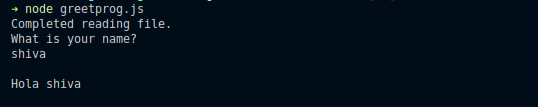
\includegraphics[width = \textwidth]{Non-block/op1.png}
\end{figure}
\begin{figure}[h]
    \centering
    
\includegraphics[width = \textwidth]{Non-block/op2.png}
\end{figure}
\begin{figure}[h]
    \centering
    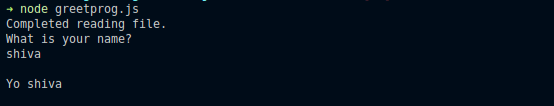
\includegraphics[width = \textwidth]{Non-block/op3.png}
\end{figure}


\hrule
\newpage

\subsection*{\underline{\textbf{Server greeting}}}
%Objective
\subsection*{\flushleft{Objective:}}
\begin{flushleft}
    Write a Node.js program that reads all the greetings as before. When all the greetings are loaded, it creates 
    a server listening on port number 8080. On request,  it  checks  for  whether  there  is  a name value  in  the  
    query string. If there isn’t, the value of query.name will be undefined.
\end{flushleft}

%Code
\subsection*{\flushleft{Code:}}
\subsubsection*{\flushleft{greetings.txt:}}
\begin{flushleft}
\lstinputlisting{Server/greetings.txt}
\end{flushleft}

\subsubsection*{{\flushleft{JavaScript:}}}
\begin{flushleft}
    \lstinputlisting[language = HTML]{Server/web.js}
\end{flushleft}

\newpage
%Output
\subsection*{\flushleft{Output:}}
\begin{figure}[h]
    \centering
    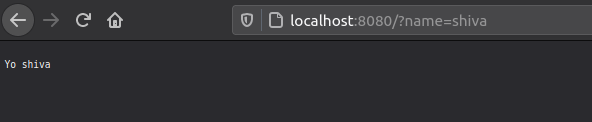
\includegraphics[width = \textwidth]{Server/op1.png}
\end{figure}
\begin{figure}[h]
    \centering
    
\includegraphics[width = \textwidth]{Server/op2.png}
\end{figure}
\begin{figure}[h]
    \centering
    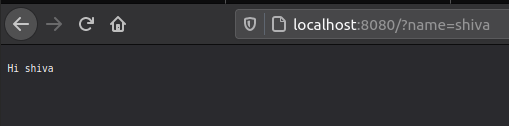
\includegraphics[width = \textwidth]{Server/op3.png}
\end{figure}
\newpage
\begin{figure}[h]
    \centering
    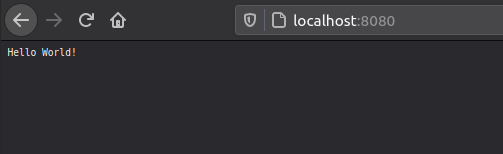
\includegraphics[width = \textwidth]{Server/op4.png}
\end{figure}

\hrule
\end{document}